%\packagelist
\documentclass[10pt]{article}
\usepackage[top=3cm, bottom=3cm, outer=3cm, inner=3cm]{geometry}
\usepackage{multicol}
\usepackage{graphicx}
\usepackage{url}
%\usepackage{cite}
\usepackage{hyperref}
\usepackage{array}
%\usepackage{multicol}
\newcolumntype{x}[1]{>{\centering\arraybackslash\hspace{0pt}}p{#1}}
\usepackage{natbib}
\usepackage{pdfpages}
\usepackage{multirow}
\usepackage[normalem]{ulem}

\useunder{\uline}{\ul}{}
\usepackage{svg}
\usepackage{xcolor}
\usepackage{listings}

\lstdefinestyle{ascii-tree}{
    literate={├}{|}1 {─}{--}1 {└}{+}1 
  }
\lstset{basicstyle=\ttfamily,
  showstringspaces=false,
  commentstyle=\color{red},
  keywordstyle=\color{blue}
}
%\usepackage{booktabs}
\usepackage{caption}
\usepackage{subcaption}
\usepackage{float}
\usepackage{array}

\newcolumntype{M}[1]{>{\centering\arraybackslash}m{#1}}
\newcolumntype{N}{@{}m{0pt}@{}}


%%%%%%%%%%%%%%%%%%%%%%%%%%%%%%%%%%%%%%%%%%%%%%%%%%%%%%%%%%%%%%%%%%%%%%%%%%%%
%%%%%%%%%%%%%%%%%%%%%%%%%%%%%%%%%%%%%%%%%%%%%%%%%%%%%%%%%%%%%%%%%%%%%%%%%%%%
\newcommand{\itemEmail}{rchambillap@unsa.edu.pe}
\newcommand{\itemStudent}{Chambilla Perca Ricardo Mauricio}
\newcommand{\itemCourse}{Programacion Web 2}
\newcommand{\itemCourseCode}{1701213}
\newcommand{\itemSemester}{III}
\newcommand{\itemUniversity}{Universidad Nacional de San Agustín de Arequipa}
\newcommand{\itemFaculty}{Facultad de Ingeniería de Producción y Servicios}
\newcommand{\itemDepartment}{Departamento Académico de Ingeniería de Sistemas e Informática}
\newcommand{\itemSchool}{Escuela Profesional de Ingeniería de Sistemas}
\newcommand{\itemAcademic}{2024 - A}
\newcommand{\itemInput}{Del 8 de Mayo 2024}
\newcommand{\itemOutput}{Al 15 de Mayo 2024}
\newcommand{\itemPracticeNumber}{1}
\newcommand{\itemTheme}{Docker}
%%%%%%%%%%%%%%%%%%%%%%%%%%%%%%%%%%%%%%%%%%%%%%%%%%%%%%%%%%%%%%%%%%%%%%%%%%%%
%%%%%%%%%%%%%%%%%%%%%%%%%%%%%%%%%%%%%%%%%%%%%%%%%%%%%%%%%%%%%%%%%%%%%%%%%%%%

\usepackage[english,spanish]{babel}
\usepackage[utf8]{inputenc}
\AtBeginDocument{\selectlanguage{spanish}}
\renewcommand{\figurename}{Figura}
\renewcommand{\refname}{Referencias}
\renewcommand{\tablename}{Tabla} %esto no funciona cuando se usa babel
\AtBeginDocument{%
	\renewcommand\tablename{Tabla}
}

\usepackage{fancyhdr}
\pagestyle{fancy}
\fancyhf{}
\setlength{\headheight}{30pt}
\renewcommand{\headrulewidth}{1pt}
\renewcommand{\footrulewidth}{1pt}
\fancyhead[L]{\raisebox{-0.2\height}{
\includegraphics[width=3cm]{./img/logo_episunsa.png}}}
\fancyhead[C]{\fontsize{7}{7}\selectfont	\itemUniversity \\ \itemFaculty \\ \itemDepartment \\ \itemSchool \\ \textbf{\itemCourse}}
\fancyhead[R]{\raisebox{-0.2\height}{
\includegraphics[width=1.2cm]{./img/logo_abet}}}
\fancyfoot[L]{Estudiante Ricardo Ch}
\fancyfoot[C]{\itemCourse}
\fancyfoot[R]{Página \thepage}

% para el codigo fuente 
\usepackage{listings}
\usepackage{color, colortbl}
\definecolor{numberOrange}{RGB}{235, 126, 9}
\definecolor{mygreen}{RGB}{40, 194, 6}
\definecolor{dkgreen}{rgb}{0,0.6,0}
\definecolor{myblue}{RGB}{57, 118, 189}
\definecolor{gray}{rgb}{0.156,0.146,0.135}
\definecolor{mygray}{RGB}{135, 135, 135}
\definecolor{mauve}{rgb}{0.58,0,0.82}
\definecolor{codebackgroundCode}{RGB}{10, 10, 20}
\definecolor{codebackgroundBash}{rgb}{0.95, 0.95, 0.92}
\definecolor{tablebackground}{rgb}{0.8, 0, 0}


\lstdefinestyle{java}{frame=tb,
	language=Java,
	showstringspaces=false,
	columns=flexible,
	basicstyle={\footnotesize\ttfamily\color[RGB]{255,255,255}},
	numberstyle=\color{mygray},
	numbers=left, 
	keywordstyle=\color{myblue},
	morekeywords={String, System},
	commentstyle=\color{mygray},
	stringstyle=\color{mygreen},
	breaklines=true,
	breakatwhitespace=true,
	tabsize=2,
	backgroundcolor= \color{codebackgroundCode},
	showspaces=false,
	showtabs=false,
	showlines=false,
}

\lstdefinestyle{mybash}{frame=tb,
	language=bash,
	showstringspaces=false,
	columns=flexible,
	keepspaces=true,
	basicstyle={\small\ttfamily},
	numberstyle=\color{mygray},
	keywordstyle=\color{myblue},
	morekeywords={java, javac},
	commentstyle=\color{mygray},
	stringstyle=\color{mygreen},
	breaklines=true,
	breakatwhitespace=true,
	tabsize=2,
	backgroundcolor= \color{codebackgroundBash},
	showspaces=false,
	showtabs=false,
	showlines=false,
}

\begin{document}
\lstset{
    literate={─}{--}2 {├}{|---}2 {└}{|---}2
}
	\vspace*{10px}
	
	\begin{center}	
		\fontsize{17}{17} \textbf{ Informe de Laboratorio N}
	\end{center}
	\centerline{\textbf{\Large Tema: \itemTheme}}
	%\vspace*{0.5cm}	

	\begin{flushright}
		\begin{tabular}{|M{2.5cm}|N|}
			\hline
			\rowcolor{tablebackground}
			\color{white} \textbf{Nota}  \\
			\hline 
			     \\[30pt]
			\hline 			
		\end{tabular}
	\end{flushright}	

	\begin{table}[H]
		\begin{tabular}{|x{4.7cm}|x{4.8cm}|x{4.8cm}|}
			\hline 
			\rowcolor{tablebackground}
			\color{white} \textbf{Estudiante} & \color{white}\textbf{Escuela}  & \color{white}\textbf{Asignatura}   \\
			\hline 
			{\itemStudent \par \itemEmail} & \itemSchool & {\itemCourse \par Semestre: \itemSemester \par Código: \itemCourseCode}     \\
			\hline 			
		\end{tabular}
	\end{table}		
	
	\begin{table}[H]
		\begin{tabular}{|x{4.7cm}|x{4.8cm}|x{4.8cm}|}
			\hline 
			\rowcolor{tablebackground}
			\color{white}\textbf{Laboratorio} & \color{white}\textbf{Tema}  & \color{white}\textbf{Duración}   \\
			\hline 
			\itemPracticeNumber & \itemTheme & 08  \\
			\hline 
		\end{tabular}
	\end{table}
	
	\begin{table}[H]
		\begin{tabular}{|x{4.7cm}|x{4.8cm}|x{4.8cm}|}
			\hline 
			\rowcolor{tablebackground}
			\color{white}\textbf{Semestre académico} & \color{white}\textbf{Fecha de inicio}  & \color{white}\textbf{Fecha de entrega}   \\
			\hline 
			\itemAcademic & \itemInput &  \itemOutput  \\
			\hline 
		\end{tabular}
	\end{table}
	
	
	\section{Ejercicios propuestos}
	Crear un contenedor en Docker basado en ubuntu 20.04:
	Especificaciones del Lab 01 
	
	\subsection*{Instale el servidor web Apache HTTP server 2.x }
	En mi caso, el trabajo final de programacion web 1, fue realizado con el servidor NGINX, que similiar a Apache, despliega contenido estatico y puede ejecutar
	CGIS. Este software lo instalo en mi imagen a travez de el archivo de DockerFile

	\begin{lstlisting}
		RUN apt-get update
		RUN apt-get install -y nginx
		RUN apt-get install -y fcgiwrap
	\end{lstlisting}
	
	\subsection{Instale cualquiera de estos lenguajes de programación: PHP, Perl, Python.\newline Configure el servidor web para que interprete uno de los lenguajes de programación.}
	De la misma forma, para el lenguaje de programacion que utilizamos fue Perl, y en el dockerfile en el que estoy mi contenedor saca la imagen se encuentra las instrucciones para la 
	instalacion de estas dependencias
	
	\begin{lstlisting}
		RUN apt-get install -y perl
		RUN apt-get install -y cpanminus
		# Lets make this inside the container
		# RUN cpan CGI
		# RUN cpan DBI
		# RUN cpan JSON
		# RUN cpan CGI::Session
	\end{lstlisting}

	Como se puede ver eh comentado la instalacion de los modulos de Perl que utilizamos para realizar la pagina web.

	\subsection{Instale cualquiera de los servidores de base de datos: MySQL, MariaDB, PostgreSQL.\newline
	Instale el servidor Open SSH Server. Envíe archivos al servidor: imágenes, css, js, etc.\newline}

	En el dockerfile tambien se instala la base de datos MariaDB.

	\begin{lstlisting}
		RUN apt-get install -y mariadb-server
	\end{lstlisting}

	\subsection{Cree un usuario pweb2 con contraseña: 12345678. \newline
	Otorgue permisos al usuario para acceder a la aplicación web. (Read/Write) \newline}

	Esta operacion se realizo a travez del terminal del container una vez creado la imagen y corriendo,
	En resumen el dockerfile que utilizo para crear la imagen se ve tal que asi:

	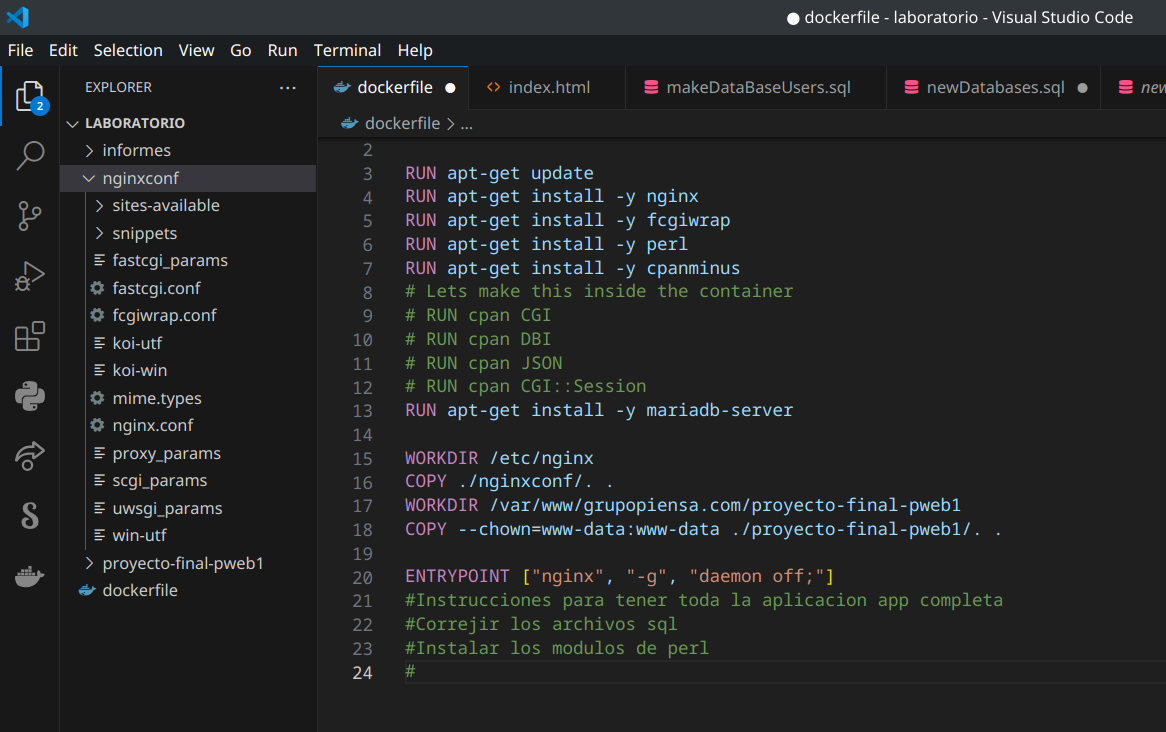
\includegraphics[scale=0.4]{./img/lab1_1.png}
	
	Una vez adentro del terminal del contenedor puedo comenzar los procesos de MariaDB asi como el servicio de fcgiwrap
	el cual me permite ejecutar cgi en servidores estaticos administrados por nginx.\newline \newline

	\begin{lstlisting}[style=mybash]
		docker run -dp 8000:80 nginxserver
		docker exec -it mystifying_ellis /bin/bash
		root@1a30749290f4:/var/www/grupopiensa.com/proyecto-final-pweb1# /etc/init.d/mariadb start
		 * Starting MariaDB database server mariadbd                                                                                                                                         [ OK ] 
		root@1a30749290f4:/var/www/grupopiensa.com/proyecto-final-pweb1# /etc/init.d/fcgiwrap start
		 * Starting FastCGI wrapper fcgiwrap                                                                                                                                                 [ OK ] 
		root@1a30749290f4:/var/www/grupopiensa.com/proyecto-final-pweb1# mysql
		Welcome to the MariaDB monitor.  Commands end with ; or \g.
		Your MariaDB connection id is 33
		Server version: 10.6.16-MariaDB-0ubuntu0.22.04.1 Ubuntu 22.04

		Copyright (c) 2000, 2018, Oracle, MariaDB Corporation Ab and others.

		Type 'help;' or '\h' for help. Type '\c' to clear the current input statement.

		MariaDB [(none)]> create database pweb1
		    -> ;
		Query OK, 1 row affected (0.001 sec)		
		MariaDB [(none)]> GRANT ALL PRIVILEGES ON pweb1.* TO 'alumno'@'%' IDENTIFIED BY 'pweb1';
		Query OK, 0 rows affected (0.015 sec)

		MariaDB [(none)]> exit
		Bye

	\end{lstlisting}

	\subsection{Finalmente implemente el trabajo final del curso de pw1 en ese contenedor. \newline
	Elabore un informe paso a paso para donde explique funcionalmente el proyecto demostrando  que se trata de un contenedor docker.\newline
	Adjunte la URL de un video donde muestre que se trata de un contenedor Docker. \newline}

	Entonces para probar mi contenedor de docker que este correctamente sirviendo los servidores de nginx voy a entrar al buscador de firefox 
	y buscar la pagina web grupopiensa, el cual esta mapeado al localhost 127.0.0.1 en el puerto 8000, el cual tiene un port forwarding
	al puerto 80 del contenedor

	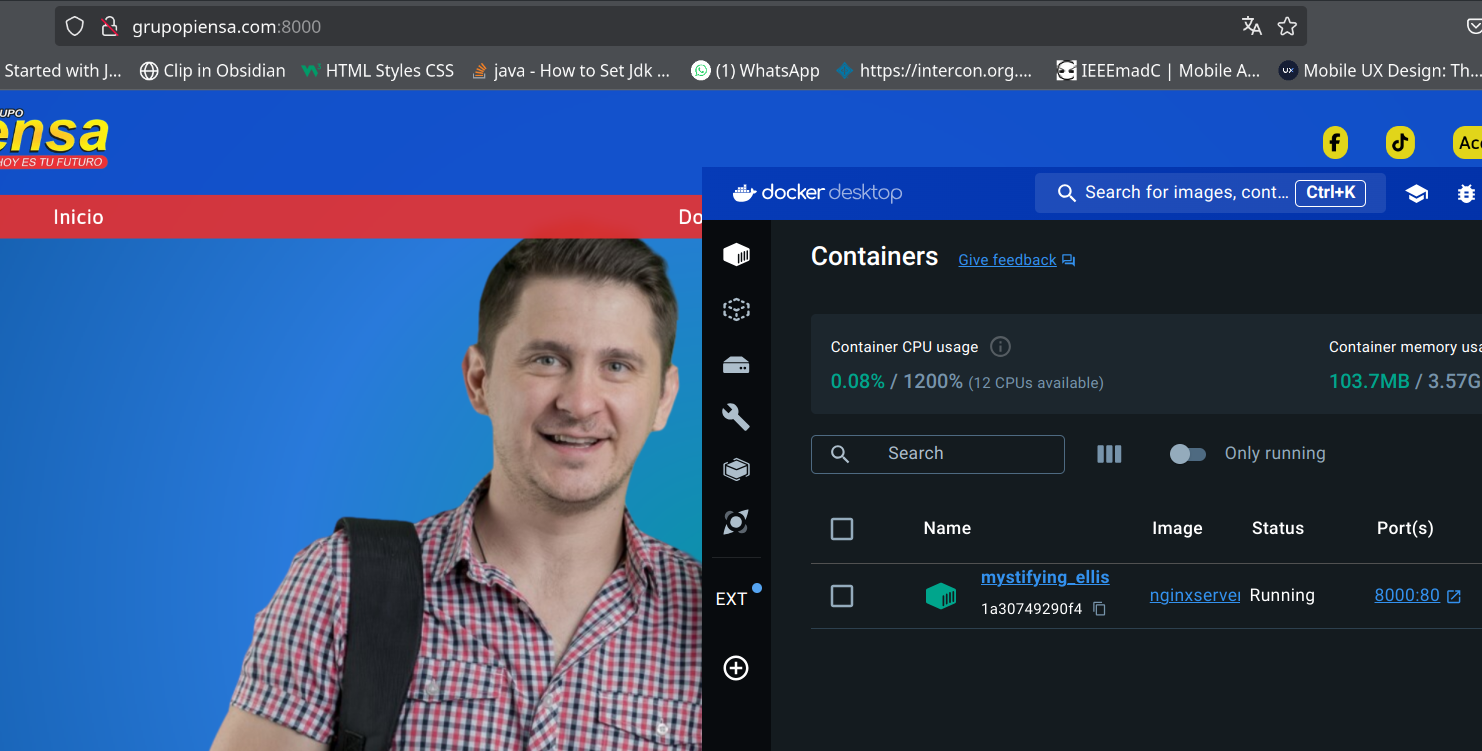
\includegraphics[scale = 0.3]{./img/lab1_2.png}
	\newline
	Aqui dejo el enlace al video de YT en el que se muestra la veracidad del uso de Docker para hostear paginas web: https://youtu.be/ERklT6IMV7E

\pagebreak

	\section{\textcolor{red}{Rúbricas}}
	
	\subsection{\textcolor{red}{Entregable Informe}}
	\begin{table}[H]
		\caption{Tipo de Informe}
		\setlength{\tabcolsep}{0.5em} % for the horizontal padding
		{\renewcommand{\arraystretch}{1.5}% for the vertical padding
		\begin{tabular}{|p{3cm}|p{12cm}|}
			\hline
			\multicolumn{2}{|c|}{\textbf{\textcolor{red}{Informe}}}  \\
			\hline 
			\textbf{\textcolor{red}{Latex}} & \textcolor{blue}{El informe está en formato PDF desde Latex,  con un formato limpio (buena presentación) y facil de leer.}   \\ 
			\hline 
			
			
		\end{tabular}
	}
	\end{table}
	
	\subsection{\textcolor{red}{Rúbrica para el contenido del Informe y demostración}}
	\begin{itemize}			
		\item El alumno debe marcar o dejar en blanco en celdas de la columna \textbf{Checklist} si cumplio con el ítem correspondiente.
		\item Si un alumno supera la fecha de entrega,  su calificación será sobre la nota mínima aprobada, siempre y cuando cumpla con todos lo items.
		\item El alumno debe autocalificarse en la columna \textbf{Estudiante} de acuerdo a la siguiente tabla:
	
		\begin{table}[ht]
			\caption{Niveles de desempeño}
			\begin{center}
			\begin{tabular}{ccccc}
    			\hline
    			 & \multicolumn{4}{c}{Nivel}\\
    			\cline{1-5}
    			\textbf{Puntos} & Insatisfactorio 25\%& En Proceso 50\% & Satisfactorio 75\% & Sobresaliente 100\%\\
    			\textbf{2.0}&0.5&1.0&1.5&2.0\\
    			\textbf{4.0}&1.0&2.0&3.0&4.0\\
    		\hline
			\end{tabular}
		\end{center}
	\end{table}	
	
	\end{itemize}
	
	\begin{table}[H]
		\caption{Rúbrica para contenido del Informe y demostración}
		\setlength{\tabcolsep}{0.5em} % for the horizontal padding
		{\renewcommand{\arraystretch}{1.5}% for the vertical padding
		%\begin{center}
		\begin{tabular}{|p{2.7cm}|p{7cm}|x{1.3cm}|p{1.2cm}|p{1.5cm}|p{1.1cm}|}
			\hline
    		\multicolumn{2}{|c|}{Contenido y demostración} & Puntos & Checklist & Estudiante & Profesor\\
			\hline
			\textbf{1. GitHub} & Hay enlace URL activo del directorio para el  laboratorio hacia su repositorio GitHub con código fuente terminado y fácil de revisar. &2 &X &2 & \\ 
			\hline
			\textbf{2. Commits} &  Hay capturas de pantalla de los commits más importantes con sus explicaciones detalladas. (El profesor puede preguntar para refrendar calificación). &4 &X &4 & \\ 
			\hline 
			\textbf{3. Código fuente} &  Hay porciones de código fuente importantes con numeración y explicaciones detalladas de sus funciones. &2 &X &1 & \\ 
			\hline 
			\textbf{4. Ejecución} & Se incluyen ejecuciones/pruebas del código fuente  explicadas gradualmente. &2 &X &1 & \\ 
			\hline			
			\textbf{5. Pregunta} & Se responde con completitud a la pregunta formulada en la tarea.  (El profesor puede preguntar para refrendar calificación).  &2 &X &2 & \\ 
			\hline	
			\textbf{6. Fechas} & Las fechas de modificación del código fuente estan dentro de los plazos de fecha de entrega establecidos. &2 &X &0 & \\ 
			\hline 
			\textbf{7. Ortografía} & El documento no muestra errores ortográficos. &2 &X &2 & \\ 
			\hline 
			\textbf{8. Madurez} & El Informe muestra de manera general una evolución de la madurez del código fuente,  explicaciones puntuales pero precisas.  &4 &X &4 & \\ 
			\hline
			\multicolumn{2}{|c|}{\textbf{Total}} &20 & &16 & \\ 
			\hline
		\end{tabular}
		%\end{center}
		%\label{tab:multicol}
		}
	\end{table}
	
\clearpage

\section{Referencias}
\begin{itemize}			
	\item \url{https://drive.google.com/file/d/19hjCsMtViypEj3cOPRF_cflH1r8r9vBn/view?usp=sharing}
\end{itemize}	
	
%\clearpage
%\bibliographystyle{apalike}
%\bibliographystyle{IEEEtranN}
%\bibliography{bibliography}
			
\end{document}